% =========================================================================== %

\begin{frame}[t,plain]
\titlepage
\end{frame}

% =========================================================================== %

\begin{frame}{Recap}
%
\begin{columns}[T]
\column{.5\linewidth}
\begin{itemize}
\item Decorators in general
	\begin{itemize}
	\item Functions that compute functions from functions
	\item Alter (add) behaviour of decorated function
	\item Often: Debug, Timing, Caching
	\item \texttt{@}-Syntax
	\end{itemize}
\item Parametrized Decorators
	\begin{itemize}
	\item Compute an apt decorator first
	\item Three levels of nested functions
	\end{itemize}
\end{itemize}
%
\column{.5\linewidth}
\begin{itemize}
\item Stacked Decorators
	\begin{itemize}
	\item Decorate a decorated function
	\item Multiple \texttt{@}-lines
	\item Or \texttt{symbol = deco1(deco2(func))}
	\end{itemize}
\item Properties
	\begin{itemize}
	\item \texttt{@property} and \texttt{@x.setter} decorators
	\item Functions will be called when accessed like variables
	\end{itemize}
\item \texttt{functools}
	\begin{itemize}
	\item Decorator \texttt{wraps} to maintain hidden variables
	\end{itemize}
\end{itemize}

\end{columns}
%
\begin{center}
	\emph{Any Questions?}
\end{center}
%
\end{frame}

% =========================================================================== %

\begin{frame}
%
\begin{columns}[T]
\column{.5\linewidth}
\begin{center}
	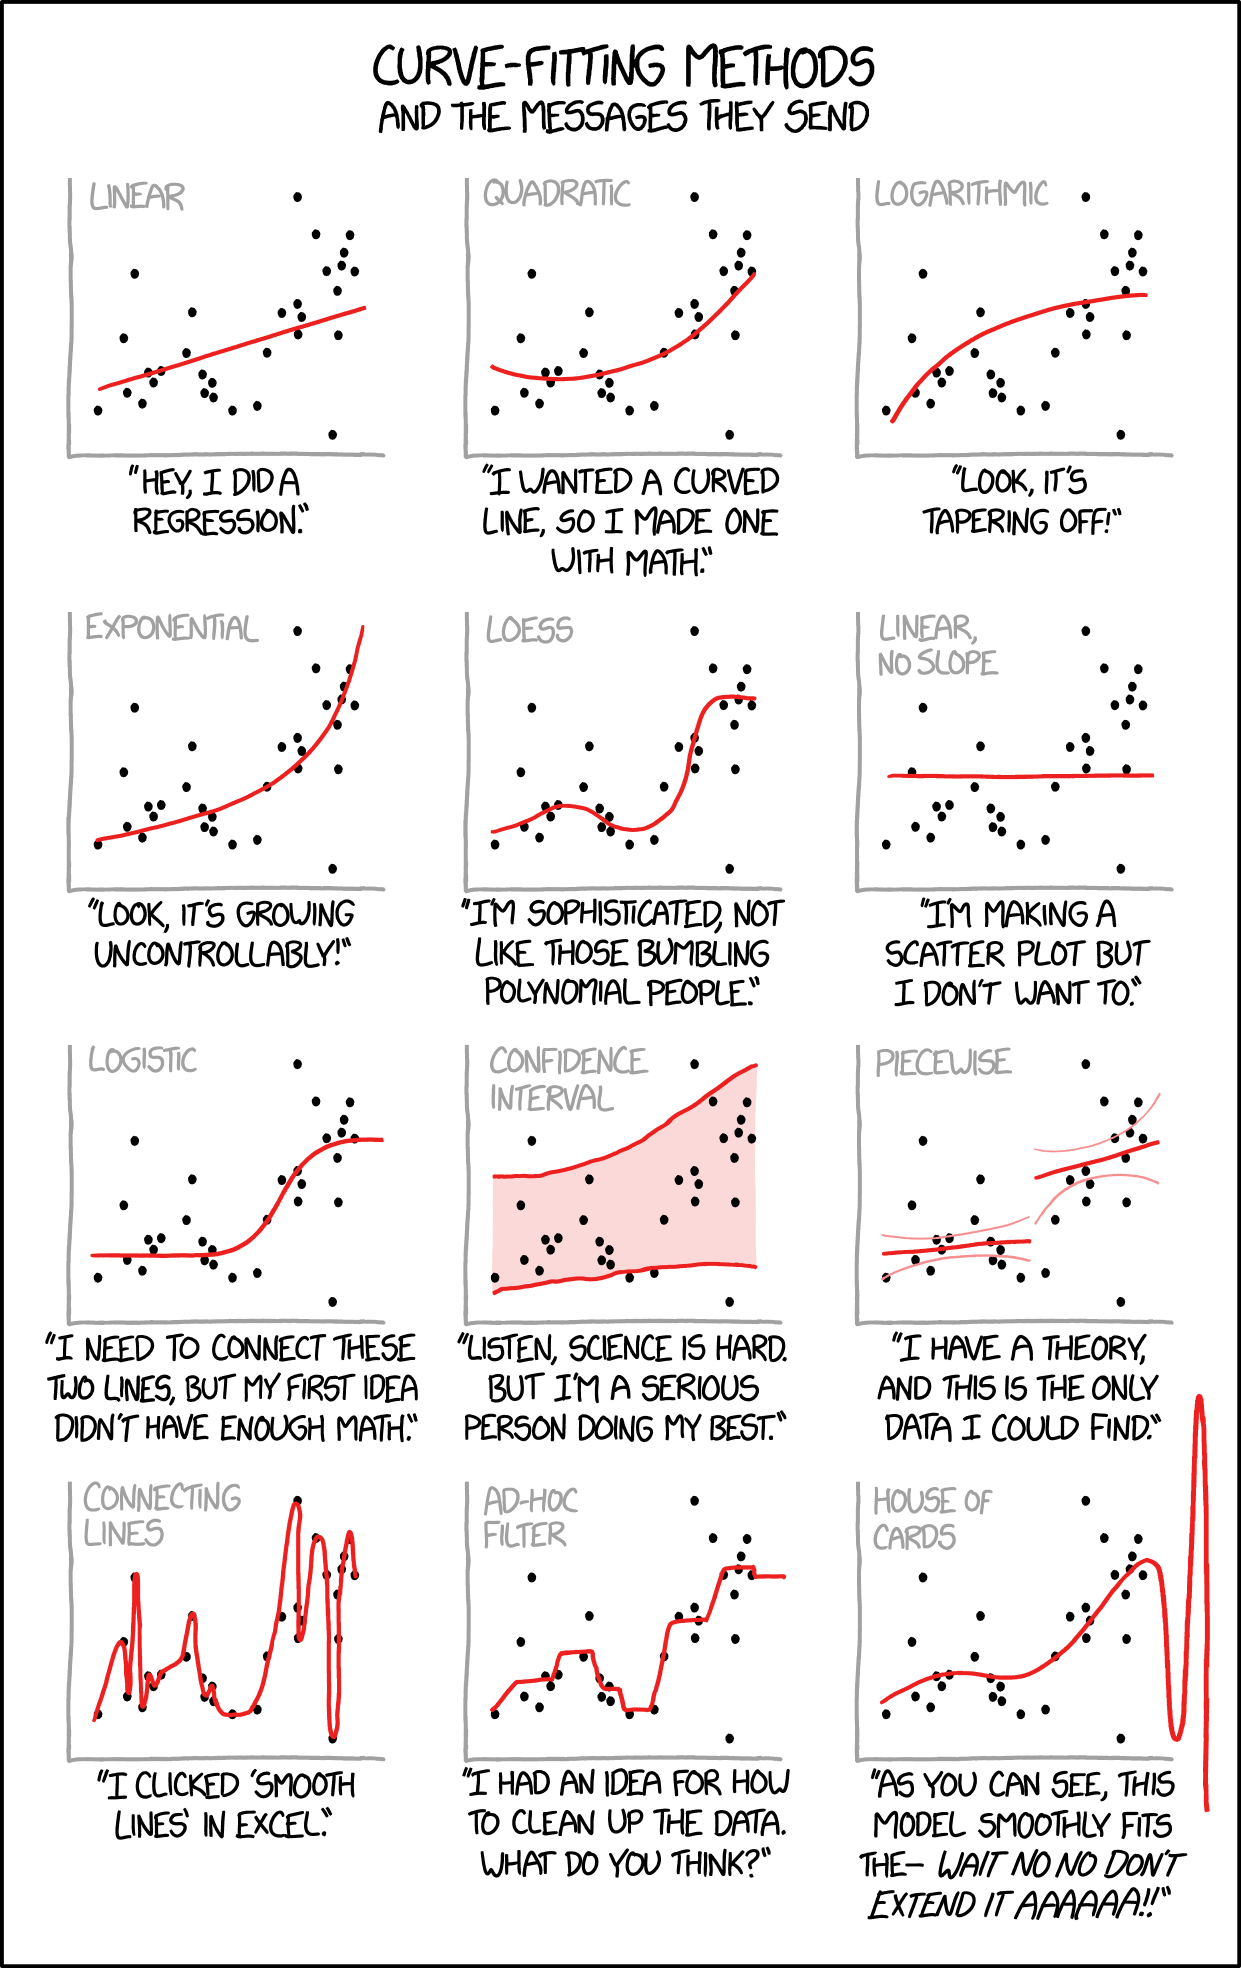
\includegraphics[width=.67\linewidth]{./gfx/xkcd-curveFitting}
\end{center}
%
\column{.5\linewidth}
\begin{Large}
	{Curve-Fitting}
\end{Large}
%
\begin{center}
	\vspace{60pt}
	\emph{Cauchy-Lorentz: \enquote{Something alarmingly mathematical is happening, and you should probably pause to Google my name and check what field I originally worked in.}}

	\vspace{6pt}
	Source: \url{https://xkcd.com/2048/}
\end{center}
\end{columns}
%
\end{frame}

% =========================================================================== %

\begin{frame}[fragile]{SciPy}
%
\begin{itemize}
\item \emph{SciPy (pronounced \enquote{Sigh Pie}) is open-source software for mathematics, science, and engineering.}
\item Installation
	\begin{itemize}
	\item Most likely: Installed with Anaconda
	\item Windows, Mac: Anaconda Shell Command:\\
		{\scriptsize \texttt{python -m pip install --user numpy scipy matplotlib pandas sympy nose}}
	\item Linux: Shell Command:\\
		{\scriptsize \texttt{sudo apt-get install python3-numpy python3-scipy python3-matplotlib python3-pandas python3-sympy python3-nose}} \\
		or\\
		{\scriptsize \texttt{sudo pip3 install --user numpy scipy matplotlib pandas sympy nose}}
	\item Upgrade may be needed
	\end{itemize}
\item Links
	\begin{itemize}
	\item \url{https://docs.scipy.org/doc/scipy/reference/index.html}
	\item \texttt{https://scipy.org/install.html}
	\end{itemize}
\end{itemize}
%
\end{frame}

% =========================================================================== %

\begin{frame}[fragile]
%
\begin{columns}[T]
\column{.5\linewidth}
\begin{Large}
	{Constants}
	\vspace{6pt}
\end{Large}
%
\begin{itemize}
\item Direct access
	\begin{itemize}
	\item \texttt{scipy.pi}
	\item \texttt{scipy.constants.golden}\\
	 (golden ratio, $\frac{1 + \sqrt{5}}{2} \approx 1.618$)
	\item \texttt{scipy.constants.c}, \texttt{scipy.constants.h}, \texttt{scipy.constants.hbar}, ...
	\item SI units
	\end{itemize}
\item Access via functions
	\begin{itemize}
	\item \texttt{scipy.constants.value}: numerical value
	\item \texttt{scipy.constants.unit}: physical dimension as string
	\item \texttt{scipy.constants.precision}: relative error of numerical value
	\end{itemize}
\end{itemize}
%
\column{.5\linewidth}
\begin{codebox}[Example: SciPy Constants]
\begin{minted}[fontsize=\scriptsize]{python3}
from scipy import constants as sc

print(sc.pi)
print(
  sc.value    ('Avogadro constant'), "±",
  sc.precision('Avogadro constant'),
  sc.unit     ('Avogadro constant'))
print()
\end{minted}
\end{codebox}
%
\begin{cmdbox}[Output: SciPy Constants]
\begin{minted}[fontsize=\scriptsize]{text}
3.141592653589793
6.02214076e+23 ± 0.0 mol^-1
\end{minted}
\end{cmdbox}
%
See Documentation\\
	\scriptsize \url{https://docs.scipy.org/doc/scipy/reference/constants.html#module-scipy.constants}
\end{columns}
%
\end{frame}

% =========================================================================== %

\begin{frame}[fragile]
%
\begin{columns}[T]
\column{.5\linewidth}
\begin{Large}
	{Special Functions}
	\vspace{6pt}
\end{Large}
%
\begin{itemize}
\item \emph{Huge} collection of (more or less) common functions
	\begin{itemize}
	\item Airy functions
	\item Elliptic functions and integrals
	\item Bessel functions
		\begin{itemize}
		\item Zeros of Bessel functions
		\item Integrals of Bessel functions
		\item Derivatives of Bessel functions
		\item Spherical Bessel functions
		\item Riccati-Bessel functions
		\end{itemize}
	\item Struve functions
	\item Raw statistical functions
	\item Information Theory functions
	\item Gamma and related functions
	\item Error function and Fresnel integrals
	\item Legendre functions
	\end{itemize}
\end{itemize}
%
\column{.5\linewidth}
\begin{codebox}[Example: SciPy Special Functions]
\begin{minted}[fontsize=\scriptsize]{python3}
from scipy import special as sf
# Bessel function of 1st kind in x = 0
print( sf.jv(1, 0) ) 
\end{minted}
\end{codebox}
%
\begin{itemize}
\item[]
\begin{itemize}
	\item Ellipsoidal harmonics
	\item Orthogonal polynomials
	\item Hypergeometric functions
	\item Parabolic cylinder functions
	\item Mathieu and related functions
	\item Spheroidal wave functions
	\item Kelvin functions
	\item Combinatorics
	\item Lambert W and related functions
\end{itemize}
\end{itemize}
%
See Documentation\\
	\scriptsize \url{https://docs.scipy.org/doc/scipy/reference/special.html#module-scipy.special}
\end{columns}
%
\end{frame}

% =========================================================================== %

\begin{frame}[fragile]
%
\begin{columns}[T]
\column{.5\linewidth}
\begin{Large}
	{Integrals}
	\vspace{6pt}
\end{Large}
%
\begin{itemize}
\item Numerical Integration for various scenarios
\item Base case: 
	\begin{itemize}
	\item $\displaystyle \int_{a}^{b} \dd{x} \; f(x)$
	\item Scalar valued function in one scalar variable
	\end{itemize}
\item \texttt{scipy.integrate.quad}
	\begin{itemize}
	\item Needs $f$, $a$, $b$
	\item Returns \inPy{tuple} of (integral, error)
	\item Optional: Further Parameters to $f$:\\
		$f = f(x, y, z)$ \\
		\Thus pass $(y, z)$ as \inPy{tuple args}
	\item Optional: Accuracy, and others
	\item $\infty$ is \texttt{scipy.inf}
	\end{itemize}
\end{itemize}
%
\column{.5\linewidth}
\begin{codebox}[Example: Simple Integral]
\begin{minted}[fontsize=\scriptsize]{python3}
import math
from scipy import integrate as integrate

f = lambda x : math.sin(x)

print( integrate.quad(f, 0, math.pi) )
\end{minted}
\end{codebox}
%
\begin{cmdbox}[Output: Simple Integral]
\begin{minted}[fontsize=\scriptsize]{text}
(2.0, 2.220446049250313e-14)
\end{minted}
\end{cmdbox}
%
See Documentation\\
	\scriptsize \url{https://docs.scipy.org/doc/scipy/reference/generated/scipy.integrate.quad.html#scipy.integrate.quad}
\end{columns}
%
\end{frame}

% =========================================================================== %

\begin{frame}[fragile]{Integrals: Variants}
%
%
\begin{itemize}
\item \texttt{dblquad}
	\begin{itemize}
	\item $\displaystyle \int_{a}^{b} \dd{x} \int_{g(x)}^{h(x)} \dd{y} \; f(x, y)$
	\item Documentation:
		{\scriptsize \url{https://docs.scipy.org/doc/scipy/reference/generated/scipy.integrate.quad.html#scipy.integrate.quad}}
	\end{itemize}
\item \texttt{tplquad}
	\begin{itemize}
	\item $\displaystyle \int_{a}^{b} \dd{x} \int_{g(x)}^{h(x)} \dd{y} \int_{q(x, y)}^{r(x, y)} \dd{z} \;f(x, y, z)$
	\item Documentation:
		{\scriptsize \url{https://docs.scipy.org/doc/scipy/reference/generated/scipy.integrate.tplquad.html#scipy.integrate.tplquad}}
	\end{itemize}
\item \texttt{quad\_vec}
	\begin{itemize}
	\item $\displaystyle \int_{a}^{b} \dd{x} \;\vec{f}(x)$
	\item Documentation: 
		{\scriptsize \url{https://docs.scipy.org/doc/scipy/reference/generated/scipy.integrate.quad_vec.html#scipy.integrate.quad_vec}}
	\end{itemize}
\end{itemize}
%
\end{frame}

% =========================================================================== %

\begin{frame}[fragile]
%
\begin{minipage}[b]{.7\linewidth}
\begin{codebox}[Example: Double Integral]%, width=.70\linewidth, nobeforeafter]
\begin{minted}[linenos, fontsize=\scriptsize]{python3}
import scipy
import numpy as np
import matplotlib.pyplot as plt
from mpl_toolkits.mplot3d import Axes3D

gaussian = lambda x, y, a : np.exp(-(x**2 + y**2) / a )
alpha = 1

x = y = np.linspace(-2, 2, 101)
X, Y = np.meshgrid(x, y)
Z = gaussian(X, Y, alpha)

fig = plt.figure( figsize=(8,8))
drw = fig.add_subplot(projection='3d')
drw.plot_surface(X, Y, Z)
fig.show()

print( scipy.integrate.dblquad(gaussian,
                               -scipy.inf, scipy.inf,
                               -scipy.inf, scipy.inf,
                               args=(alpha,)) )
\end{minted}
\end{codebox}
\end{minipage}
%
\begin{minipage}[b]{.29\linewidth}
\[
	f_\alpha(x, y)
=
	\exp( -\frac
	{x^2 + y^2}
	{\alpha} )
\]
%
\begin{tcolorbox}[title=Output]%, width=.29\linewidth, nobeforeafter]
	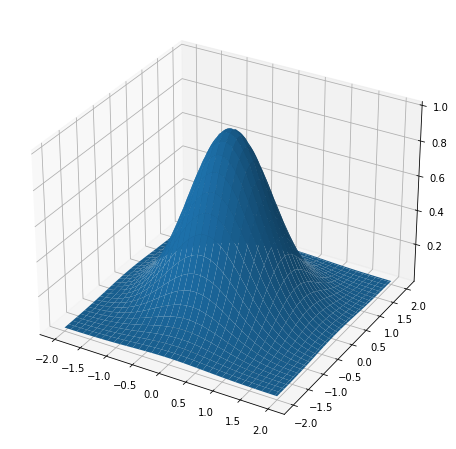
\includegraphics[width=\linewidth]{./gfx/gaussian-2D}
\end{tcolorbox}
%
\begin{cmdbox}[Output]%, width=.29\linewidth, nobeforeafter]
\begin{minted}[fontsize=\scriptsize]{text}
(3.1415926535898,
 2.5173086737433e-08)
\end{minted}
\end{cmdbox}
\end{minipage}
%
\end{frame}

% =========================================================================== %

\begin{frame}{Integrals: Optimization}
%
\begin{itemize}
\item Numerical Integration: weighted sum of discrete points
\item Invocation of $f$ for each single point
\item Can take \emph{a lot} of overhead time
\item Alternative: Vectorization
	\begin{itemize}
	\item Use NumPy functions to compute points in one singe call
	\item Pass a NumPy array to the integrator
	\item Use one of many vector integrators
	\end{itemize}
\item We'll have a look at the trapezoid (\texttt{trapz}), Simpson (\texttt{simp}) and Romberg (\texttt{romb}) method
\end{itemize}
%
\end{frame}

% =========================================================================== %

\begin{frame}[fragile]{Vector Integrators: Interface}
%
\begin{codebox}[Syntax: Calls to Vector Integrators]
\begin{minted}[fontsize=\scriptsize]{python3}
from scipy import integrate as integrate

integrate.XXX(Y, X = None, dx = 1, axis = -1)
integrate.romb(Y, dx = 1, axis = -1)
\end{minted}
\end{codebox}
%
\begin{itemize}
\item All of them
	\begin{itemize}
	\item \texttt{Y}: vector with pre-evaluated data points
	\item \texttt{dx}: space between two data points (or weight)
	\item \texttt{axis}: number of index along which to integrate if doing several functions in a single call
	\end{itemize}
\item \texttt{trapz} and \texttt{simp} (aka \texttt{XXX} in the above syntax scheme)
	\begin{itemize}
	\item \texttt{X}: vector of x-values on which \texttt{Y} was evaluated (\texttt{dx} is then ignored)
	\end{itemize}
\item \texttt{romb}
	\begin{itemize}
	\item \texttt{Y} needs to have exactly $2^k + 1$ elements with $k \in \mathbb{N}_0$
	\end{itemize}
\end{itemize}
%
\end{frame}

% =========================================================================== %

\begin{frame}{Comparison}
%
\begin{minipage}{.3\linewidth}
	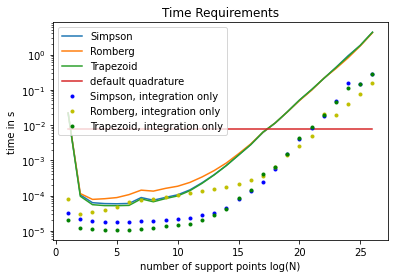
\includegraphics[width=\linewidth]{./gfx/sciPy-int-time}
\end{minipage}
\phantom{x}
\begin{minipage}{.3\linewidth}
	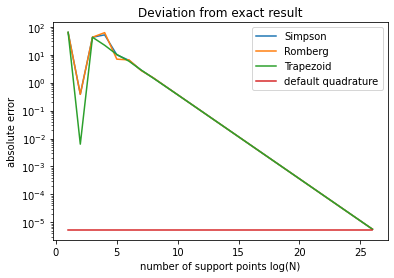
\includegraphics[width=\linewidth]{./gfx/sciPy-int-error}
\end{minipage}
\phantom{x}
\begin{minipage}{.3\linewidth}
	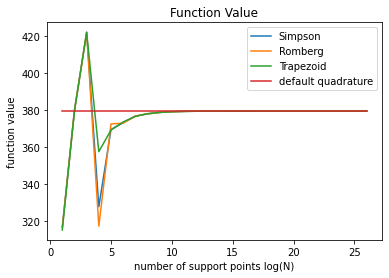
\includegraphics[width=\linewidth]{./gfx/sciPy-int-value}
\end{minipage}
{\scriptsize Test integrand: \inPy{lambda x : np.exp( np.sin(x) ) + np.exp( np.cos(x) )}}
%
\begin{itemize}
\item All three are about same speed
\item Default quadrature gives best accuracy/time ratio
\item \emph{Good enough} can be reached much faster
\item Details depend on use case. 
	\begin{itemize}
	\item Are values needed in memory anyway?
	\item How easy to do vectorized computation?
	\end{itemize}
\item See code \texttt{005-integration-b.py} on GRIPS
\end{itemize}
%
\end{frame}

% =========================================================================== %

\begin{frame}{Is it even relevant?}
%
\begin{columns}[T]
\column{.5\linewidth}
\begin{center}
	
\includegraphics[width=\linewidth]{./gfx/Dafinger-runtime}
\end{center}
%
\column{.5\linewidth}
\begin{itemize}
\item Thanks to \emph{Michael Dafinger} for this message
\item Impact of runtime depends on a plethora of factors
\item Large factors can mean virtually nothing
\item Small contributions can sum up
\item[\Thus] Make it one of your later concerns, but
\item[\Thus] Make it one of your concerns
\end{itemize}
\end{columns}
%
\end{frame}

% =========================================================================== %

\begin{frame}[fragile]{Curve Fitting}
%
\begin{itemize}
\item Got measured data as an array
\item Got an assumption: functional form, but with free parameters
\item[\Thus] \texttt{scipy.optimize.curve\_fit} finds them
\item Provide measured data as iterable
\item Provide functional form as function or lambda
	\begin{itemize}
	\item First argument: $x$
	\item Other arguments: parameters to be found
	\end{itemize}
\item Get a \inPy{tuple} as a result
	\begin{itemize}
	\item First element: NumPy-Array of parameters
	\item Covariance of parameters wrt. measured data
	\end{itemize}
\item See documentation\\
	{\scriptsize \url{https://docs.scipy.org/doc/scipy/reference/generated/scipy.optimize.curve_fit.html}}
\end{itemize}
%
\end{frame}

% =========================================================================== %

\begin{frame}[fragile]
%
\begin{codebox}[Example: Curve Fitting, width=.73\linewidth, nobeforeafter, equal height group=grpCurveFit]
\begin{minted}[linenos, fontsize=\scriptsize]{python3}
import numpy as np
import matplotlib.pyplot as plt
from scipy.optimize import curve_fit

xdata = np.linspace(0, 4, 50)
func = lambda x, a, b, c   :   a * np.exp(-b * x) + c

y = func(xdata, 2.5, 1.3, 0.5)
y_noise = 0.2 * np.random.normal(size=xdata.size)
ydata = y + y_noise
plt.plot(xdata, ydata, 'b-', label='data')

popt, pcov = curve_fit(func, xdata, ydata)

plt.plot(xdata, func(xdata, *popt), 'r-',
         label='fit: a=%5.3f, b=%5.3f, c=%5.3f' % tuple(popt))

plt.xlabel('x')
plt.ylabel('y')
plt.legend()
plt.show()
\end{minted}
\end{codebox}
%
\begin{tcolorbox}[title=Output, width=.26\linewidth, nobeforeafter, equal height group=grpCurveFit]
	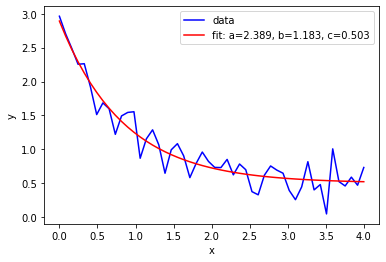
\includegraphics[width=\linewidth]{./gfx/sciPy-curve-fit}
	
	\vspace{6pt}
	\scriptsize
	Parameters found:\\
	\texttt{a = 2.47430051},\\
	\texttt{b = 1.40793326},\\
	\texttt{c = 0.49347906}
	
	\vspace{6pt}
	Syntax\\
	\texttt{'format' \% tuple}\\
	is an old but sometimes convenient way of using format strings
	
	\vspace{6pt}
	Example based on the one in the SciPy Documentation (Link on previous slide)
\end{tcolorbox}
%
\end{frame}

% =========================================================================== %

\begin{frame}{Common Issue}
%
\begin{itemize}
\item Often: \texttt{curve\_fit} fails or returns utter nonsense
\item Then often: provide an initial guess and/or limits
\item Optional parameters \texttt{p0} and \texttt{bounds}
\item \texttt{p0}
	\begin{itemize}
	\item Iterable, \eg \texttt{tuple} of values for \texttt{a, b, c, ...} that you think are reasonably close
	\item If you have no clue: Anything nonzero and in the correct \emph{order of magnitude}
	\end{itemize}
\item \texttt{bounds}
	\begin{itemize}
	\item \inPy{tuple} with two elements
	\item First element: lower boundary
	\item Can be either one single number (applies to all parameters)
	\item Or an iterable (individual values for all parameters)
	\item Second element: same for upper boundary
	\end{itemize}
\item Alternative strategy: limit range
	\begin{itemize}
	\item Instead of fit to \texttt{xdata, ydata}, fit to \texttt{xdata[start:stop], ydata[start:stop]}
	\end{itemize}
\end{itemize}
%
\end{frame}

% =========================================================================== %

\begin{frame}{Fourier Transform}
%
\begin{itemize}
\item Got: some signal
\item Want: frequency/frequencies in that signal
\item Example: sound
	\begin{itemize}
	\item Measure air pressure vs. time
	\item Want frequencies and amplitudes
	\end{itemize}
\item \emph{Fast Fourier Transform}: Matrix operation that efficiently computes FT of a signal \emph{vector}
\item SciPy offers many helpers for such problems
	\begin{itemize}
	\item Forward and inverse transformation
	\item Different norms
	\item 1D, 2D, ND transform
	\item Sine and Cosine transform
	\end{itemize}
\item Documentation\\
	{\scriptsize \url{https://docs.scipy.org/doc/scipy/reference/fft.html}}
\end{itemize}
%
\end{frame}

% =========================================================================== %

\begin{frame}[fragile]{Fast Fourier Transform: Data Types}
%
\begin{codebox}[Beispiel: Title goes here]
\begin{minted}[linenos, fontsize=\scriptsize]{python3}
A_e = scipy.fft.fft(Y, norm="ortho")   # complex valued
A_s = scipy.fft.dst(Y, norm="ortho")   # real valued, discrete sine transform
A_c = scipy.fft.dct(Y, norm="ortho")   # real valued, discrete cosine transform
\end{minted}
\end{codebox}
%
\begin{itemize}
\item Input vector: measured data, evenly spaced ($f_k = f(k \Delta t), k \in \mathbb{Z}$)
\item Optional input: norm: string, \inPy{"forward"}, \inPy{"ortho"}, \inPy{"backward"} (defines prefactor)
\item Output vector: spectrum, length same as input vector
\item Frequency associated with amplitude \texttt{A\_x[k]}: $\frac{k}{P \cdot 2 \pi}$ where $P$: number of periods in the signal
\item Output holds some \enquote{noise} due to discrete implementation
\item Inverse restores the exact signal
\end{itemize}
%
\end{frame}

% =========================================================================== %

\begin{frame}[fragile]
%
\begin{codebox}[Example: Discrete Sine Transform, width=.63\linewidth, nobeforeafter, equal height group=grpDST]
\begin{minted}[linenos, fontsize=\scriptsize]{python3}
import scipy
import numpy as np
import matplotlib.pyplot as plt

N = 6280
P = 4
X = np.linspace(0, P * 2 * np.pi, N)
Y = np.sin(np.pi * X) + .3 * np.sin(5 * np.pi * X)

A = scipy.fft.dst(Y, norm="ortho")
W = [k / (P * 2 * np.pi) for k in range(len(A))]

fig = plt.figure( figsize=(5, 10) )
drw = fig.add_subplot(211)
drw.set_xlabel("time t")
drw.set_ylabel("signal intensity")
drw.plot(X, Y)
drw = fig.add_subplot(212)
drw.set_xlabel("angular frequency $\omega$")
drw.set_ylabel("signal amplitude")
drw.plot(W[:100], A[:100])
plt.show()
\end{minted}
\end{codebox}
%
\begin{tcolorbox}[title=Output, width=.36\linewidth, nobeforeafter, equal height group=grpDST]
	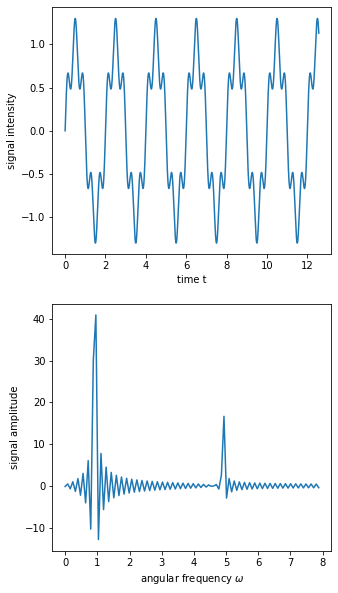
\includegraphics[width=\linewidth]{./gfx/sciPy-DST}
\end{tcolorbox}
%
\end{frame}

% =========================================================================== %

\begin{frame}{ODEs (Ordinary differential equations)}
%
Recap: First order ODE:
\begin{align*}
	y'(t) &= f(y)(t)\\
	A'(t) &= -k \cdot A(t)
\end{align*}

Higher order ODEs:
\begin{align*}
	y^{(n)}(t) &= f_{n-1}(y^{(n-1)})(t) + \ldots + f_0(y)(t)\\
	\ddot{x}(t) &= \beta \dot{x}(t) + \gamma x(t)
\end{align*}

Transform into a system of first oder ODEs:
\begin{align*}
	\begin{pmatrix}
		y^{(n)} \\
		y^{(n-1)} \\
		\hdots \\
		y^{(1)}
	\end{pmatrix}
&=
	\begin{pmatrix}
		\dv{x} y^{(n-1)} \\
		\dv{x} y^{(n-2)} \\
		\hdots \\
		f_{n-1}(y^{(n-1)})(t) + \ldots + f_0(y)(t)
	\end{pmatrix}
\end{align*}
%
\end{frame}

% =========================================================================== %\\

\begin{frame}[fragile]{Solving ODEs with SciPy}
%
\begin{itemize}
\item Function \texttt{scipy.integrate.odeint} can solve such systems of first order ODEs
\item Input:
	\begin{itemize}
	\item \texttt{func}: callable, returns vector with derivatives
	\item \texttt{y0}: initial conditions, \ie $y(t_0)$ or $y(x_0, t_0)$
	\item \texttt{t}: vector of times for which solution is to be found. \texttt{t[0]} has to be $t_0$
	\item (Optional): \texttt{args} -- parameters to \texttt{func} other than $t_0, x_0$
	\end{itemize}
\item Output:
	\begin{itemize}
	\item Matrix, size \inPy{len(t)} $\times$ \texttt{n}
	\item \texttt{result[i, n]} is $f^{(n)}(t_i)$
	\end{itemize}
\item Documentation\\
	{\scriptsize \url{https://docs.scipy.org/doc/scipy/reference/generated/scipy.integrate.odeint.html}}
\end{itemize}
%
\end{frame}

% =========================================================================== %

\begin{frame}[fragile]
%
\begin{codebox}[Example: Attenuated Pendulum, width=.57\linewidth, nobeforeafter, equal height group=grpODE]
\begin{minted}[linenos, fontsize=\scriptsize]{python3}
from scipy.integrate import odeint
import numpy as np
import matplotlib.pyplot as plt

def pend(y, t, b, c):
    theta, omega = y
    dydt = [omega, -b*omega - c*np.sin(theta)]
    return dydt

b, c = 0.25, 5.0
y0 = [np.pi - 0.1, 0.0]
t = np.linspace(0, 10, 101)

sol = odeint(pend, y0, t, args=(b, c))

plt.plot(t, sol[:, 0], 'b', label='theta(t)')
plt.plot(t, sol[:, 1], 'g', label='omega(t)')
plt.legend(loc='best')
plt.xlabel('t')
plt.grid()
plt.show()
\end{minted}
\end{codebox}
%
\begin{tcolorbox}[title=Output, width=.42\linewidth, nobeforeafter, equal height group=grpODE]
	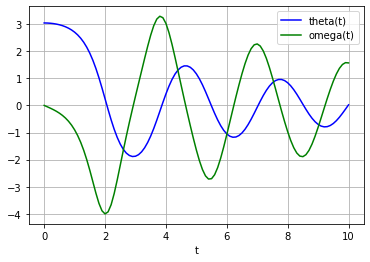
\includegraphics[width=\linewidth]{./gfx/sciPy-ODE}
	
	\vspace{6pt}
	Note that you can use this to find higher order eigenfunctions in one single call
	
	\vspace{6pt}
	Example based on the one in the SciPy Documentation (Link on previous slide)
\end{tcolorbox}
%
\end{frame}

% =========================================================================== %

\begin{frame}[fragile]
%
\begin{codebox}[Example: First Three Modes of $2^{\text{nd}}$ order ODE]
\begin{minted}[linenos, fontsize=\scriptsize]{python3}
from scipy.integrate import odeint
import numpy as np
import matplotlib.pyplot as plt

def dv (t, x_vec) :        # this essentially implements y'' = -y
    x2, x1, x0 = x_vec
    x3 = -x1
    return [x3, x2, x1]

N = 628
t = np.linspace(0, 2 * np.pi, N)
y0 = [0, 1, 0]

sol = odeint(dv, y0, t, tfirst=True)

print(sol.shape)

plt.figure()
plt.plot(t, sol[:,0], sol[:,1], sol[:,2])
plt.show()
\end{minted}
\end{codebox}
%
\end{frame}

% =========================================================================== %

\begin{frame}{ODE Solver: Under the Hood}
%
\begin{itemize}
\item Finite difference scheme
	\begin{itemize}
	\item Idea: $y(t + \Delta t) = y(t) + \Delta t \cdot y'(t) + \mathcal{O}(\Delta t)$
	\item Same idea for all orders of derivative
	\item Errors will accumulate
	\item Balance between performance ($\Delta t$ big) and accuracy ($\Delta t$ small)
	\end{itemize}
\item Translate into code
	\begin{itemize}
	\item Array \texttt{t} with apt step size
	\item Previous example: $\Delta t = \frac{t_{max} - t_0}{N}$
	\end{itemize}
\item To speed things up...
	\begin{itemize}
	\item Optimize your function \texttt{dv}
		\begin{itemize}
		\item In particular for multidimensional trajectories 
		\item Vectorization where possible!
		\end{itemize}
	\item Compute once, store in files
	\end{itemize}
\end{itemize}
%
\end{frame}

% =========================================================================== %

\begin{frame}{Notable Mentions}
%
\begin{itemize}
\item Signal Processing Module
	\begin{itemize}
	\item Convolutions, correlations
	\item Tutorial: {\scriptsize \url{https://docs.scipy.org/doc/scipy/reference/tutorial/signal.html}}
	\item Reference: {\scriptsize \url{https://docs.scipy.org/doc/scipy/reference/signal.html}}
	\end{itemize}
\item Optimization Module
	\begin{itemize}
	\item Minimization, root finding
	\item Tutorial: {\scriptsize \url{https://docs.scipy.org/doc/scipy/reference/tutorial/optimize.html}}
	\item Reference: {\scriptsize \url{https://docs.scipy.org/doc/scipy/reference/optimize.html}}
	\end{itemize}
\item Interpolation Module
	\begin{itemize}
	\item Interpolation in one and multiple dimensions
	\item Tutorial: {\scriptsize \url{https://docs.scipy.org/doc/scipy/reference/tutorial/interpolate.html}}
	\item Reference: {\scriptsize \url{https://docs.scipy.org/doc/scipy/reference/interpolate.html}}
	\end{itemize}
\item The complete documentation
	\begin{itemize}
	\item Online: {\scriptsize \url{https://docs.scipy.org/doc/scipy/reference/}}
	\item PDF: {\scriptsize \url{https://docs.scipy.org/doc/scipy/scipy-ref-1.6.1.pdf}}
	\item 3164 pages
	\end{itemize}
\end{itemize}
%
\end{frame}